% Technical report: LLM-based pathway interpretation of SynergyLM (pre-registered study, run 2026-09-29/30).
% Tables are generated from data/xai/results/analysis.json by make_tables.py; do not edit tables/*.tex by hand.
% Build: python reports/llm_interpretation/make_tables.py && cd reports/llm_interpretation && pdflatex report && pdflatex report
\documentclass[11pt]{article}
\usepackage[letterpaper,margin=0.9in]{geometry}
\usepackage[T1]{fontenc}
\usepackage{lmodern}
\usepackage{amsmath}
\usepackage{graphicx}
\usepackage{booktabs}
\usepackage{tabularx}
\usepackage{array}
\usepackage{enumitem}
\usepackage[hidelinks]{hyperref}
\setlist{nosep,leftmargin=1.4em}
\setlength{\parskip}{3pt}

\title{LLM-based pathway interpretation of SynergyLM:\\a pre-registered test of biological correctness}
\author{SynergyLM extension, technical report}
\date{1 October 2026}

\begin{document}
\maketitle

\section*{Summary}
\begin{itemize}
\item \textbf{Question.} Do SynergyLM's per-gene attributions make an LLM agent's mechanistic explanations of a drug
  combination more biologically correct than the same agent reasoning over the same knowledge graph (KG) without
  attributions? ``Correct'' means the named Reactome pathway is a cell-line-specific CRISPR dependency (DepMap) in
  the cell line being explained.
\item \textbf{Setup.} 250 synergistic and 250 antagonistic drug-pair--cell-line items; two SynergyLM variants
  (multi-omics, L1000); an attribution-guided agent and a KG-only agent, both run locally on
  \texttt{Qwen/Qwen3-32B-AWQ} with every claim checked by a mechanical verifier; deterministic no-LLM selectors as
  exploratory controls. 1,500 LLM runs.
\item \textbf{Result: null.} The primary hypothesis (H1) fails for both variants. Multi-omics: mean difference
  $+0.03$ SD (95\% CI $-0.17$ to $+0.23$, $n = 93$). L1000: $+0.22$ SD (CI $-0.09$ to $+0.57$, $n = 20$,
  underpowered). The secondary hypotheses H2 (synergy vs antagonism) and H3 (L1000 vs multi-omics) are also null.
\item \textbf{The LLM is not the bottleneck.} The guardrails worked (92--99\% of claims valid on the first try) and
  attributions were stable across seeds. But choosing the pathway from the attributions \emph{without} an LLM is no
  better than choosing a random convergent pathway, and the LLM agent does not improve on that selector. The
  attributions carry no detectable pathway-level signal about dependency. A larger or paid LLM would not change this.
\item \textbf{Likely cause.} SynergyLM's omics inputs behave as a cell-line identifier (59 cell profiles, 27,606
  features), so gene-level attributions describe which cell line it is rather than mechanism. Later experiments
  confirmed this directly (Section~\ref{sec:interpretation}).
\end{itemize}

\section{Question and hypotheses}

\begin{table}[h]
\centering
\small
\caption{Pre-registered hypotheses (plan of 2026-09-29, fixed before any agent run).}
\label{tab:hyp}
\begin{tabularx}{\linewidth}{@{}lXl@{}}
\toprule
ID & Hypothesis & Role \\
\midrule
H1 & For synergistic items, the pathway named by the attribution-guided agent has higher cell-line-specific dependency than the pathway named by the KG-only agent. Tested separately for each model variant. & Primary \\
H2 & The attribution agent's advantage is larger for synergistic than for antagonistic items. & Secondary \\
H3 & The advantage is larger with the L1000 variant (drug-side gene signal) than with the multi-omics variant. & Secondary \\
\bottomrule
\end{tabularx}
\end{table}

\textbf{Falsification rule.} If H1 fails for both variants, the attributions add no biological correctness beyond the
KG and the LLM's prior. This was declared a reportable negative result before the study ran.

\section{Methods}

\paragraph{Models.} SynergyLM~(ACM BCB 2026) predicts the ZIP synergy score of a drug pair in a cell line from frozen
MolFormer drug embeddings and cell-line omics. Two variants were explained: \emph{multi-omics} (mRNA 23,808, protein
3,171 and miRNA 627 features fused by attention) and \emph{L1000} (mRNA plus each drug's L1000 landmark signature,
978 genes). Each variant was trained with three seeds on TDC's random split (ZIP target, published hyperparameters).

\paragraph{Attributions.} Integrated Gradients (64 steps) with respect to the raw inputs, against the mean training
profile as baseline, so an attribution means ``what is distinctive about this cell line or drug''. For each channel,
$|\text{IG}|$ was summed over each Reactome pathway with at least 5 genes in the channel and compared with 10,000
size-matched random gene sets drawn from the channel's Reactome-annotated genes. Benjamini--Hochberg FDR was computed
within each channel. A pathway is \emph{attribution-supported} if its FDR is below 0.1 in at least 2 of 3 seeds. miRNA
cannot enter a pathway explanation.

\paragraph{Knowledge graph.} PrimeKG drug--protein target edges, Reactome (all levels, human, 10--300 genes: 1,733
pathways), and GO biological process as non-claimable context. KEGG was omitted pending licence terms. 100 of 129
drugs have a protein target; drugs without one (platinum compounds, most alkylators) make an item ineligible.

\paragraph{Agent.} \texttt{Qwen/Qwen3-32B-AWQ} (Apache-2.0), served locally with vLLM on one 40\,GB A100 (32,768-token
context). Thinking mode was on, with the model card's sampling settings (temperature 0.6, top-$p$ 0.95, top-$k$ 20).
A fixed per-request seed made runs reproducible, and each run had at most 25 turns. The agent receives the drug pair,
the cell line and KG tools, and must return strict JSON: a primary Reactome pathway, up to three ranked pathways, and
for each a KG path target($A$) $\to$ pathway $\leftarrow$ target($B$). A mechanical verifier outside the LLM checks
that every edge exists in the KG and, in the attribution condition, that the pathway is attribution-supported.
Rejected outputs get one retry, and the agent may abstain.

\paragraph{Conditions.}
\begin{itemize}
\item \emph{Attribution agent} (one per variant): the agent plus a tool listing the item's admissible
  attribution-supported pathways.
\item \emph{KG-only agent}: the same agent without attributions. It runs once per item because it does not depend on
  the variant.
\item Exploratory, not pre-registered:
  \begin{itemize}
  \item \emph{attribution selector}: the highest-scoring admissible pathway, chosen with no LLM;
  \item \emph{random}: the exact expected score of a uniform choice among the pair's convergent pathways.
  \end{itemize}
\end{itemize}

\paragraph{Outcome.} For pathway $P$ and cell line $C$, with Chronos gene effects from DepMap 24Q4 and at least 10
screened genes in $P$:
\[
\mathrm{dep}(P,c) = \frac{1}{|P|}\sum_{g\in P}\mathrm{Chronos}(g,c), \qquad
\mathrm{spec}(P,C) = -\,\frac{\mathrm{dep}(P,C) - \operatorname{mean}_c \mathrm{dep}(P,c)}{\operatorname{sd}_c \mathrm{dep}(P,c)}.
\]
Higher means $P$ is more selectively essential in $C$ than in other lines, which removes the advantage of pathways
that are essential everywhere. Differences in spec are in standard-deviation (SD) units.

\paragraph{Sample.} From the random-split test set:
\begin{itemize}
\item \emph{Synergy stratum}: observed ZIP in the top decile and predicted in the top quintile by both variants.
\item \emph{Antagonism stratum}: the mirror image (bottom decile, bottom quintile).
\end{itemize}
Filters:
\begin{itemize}
\item both drugs have a KG target and at least one convergent pathway;
\item neither drug uses a proxy L1000 profile;
\item the cell line has DepMap CRISPR data.
\end{itemize}
Caps: at most 8 items per cell line and 3 per drug pair. 250 items were sampled per stratum.

\paragraph{Analysis.}
\begin{itemize}
\item \textbf{H1}: per-item difference $\Delta = \mathrm{spec}_{\text{attr}} - \mathrm{spec}_{\text{KG}}$ on the synergy
  stratum, over items where both agents made a verified claim. Tests:
  \begin{itemize}
  \item a linear mixed model $\Delta \sim 1 + (1|\text{cell line}) + (1|\text{drug pair})$, Holm-corrected across the
    two variants;
  \item a 95\% cluster-bootstrap CI that resamples cell lines (2,000 resamples);
  \item the paired effect size $d_z$;
  \item a Wilcoxon signed-rank test.
  \end{itemize}
  Reported $p$-values are two-sided. The pre-registered one-sided test gives the same verdict (L1000: one-sided
  $p = 0.067$, Holm 0.13).
\item \textbf{H2}: the condition $\times$ stratum interaction in a mixed model with crossed random intercepts for cell
  line, drug pair and item.
\item \textbf{H3}: the paired difference $\Delta_{\text{L1000}} - \Delta_{\text{multi-omics}}$ on shared items.
\end{itemize}

\section{Pre-registered gates}

\begin{table}[h]
\centering
\small
\caption{Gates checked before (G0, G1) and during (G2) the agent runs.}
\label{tab:gates}
\begin{tabularx}{\linewidth}{@{}lXXl@{}}
\toprule
Gate & Criterion & Observed & Outcome \\
\midrule
G0 data & $\geq$ 32 of 59 cell lines in DepMap CRISPR and $\geq$ 250 eligible synergy items & 41 lines; 1,207 synergy and 602 antagonism items eligible & Pass \\
G1 stability & Median seed-to-seed Spearman of pathway scores $\geq$ 0.5 & 0.81 (multi-omics), 0.66 (L1000) & Pass \\
G2 verifier, pilot 1 & Attribution-agent claims valid on first try $\geq$ 0.80 (20 items, 40 runs) & 0.60; most errors claimed non-admissible pathways; one context overflow & Fail \\
G2 verifier, pilot 2 & Same, after the tool was restricted to admissible pathways & 0.95 & Pass \\
\bottomrule
\end{tabularx}
\end{table}

A power shortfall was known before the primary analysis. Only 98 of 250 synergy items (multi-omics) and 21 of 250
(L1000) had at least one admissible attribution-supported pathway, against the 240 items the power analysis assumed.
The imputed sensitivity analysis keeps all 250 items. The median item had 184 supported pathways in the multi-omics
cell channel and 7 in the L1000 channels (144 of 500 L1000 items had none). miRNA carried a median 34\% of the
multi-omics attribution mass, which no pathway explanation can use.

\section{Results}

\subsection{Agent behaviour}

\begin{table}[h]
\centering
\scriptsize
\caption{Run outcomes per condition (250 runs each). Accepted: a verified claim; abstained: no admissible pathway
claimed; rejected: failed verification after the retry. First-try valid: the fraction of first submissions passing
the verifier.}
\label{tab:behaviour}
\resizebox{\linewidth}{!}{\begin{tabular}{@{}llrrrrrr@{}}
\toprule
Condition & Stratum & Accepted & Abstained & Rejected & First-try valid & Turns & Output tokens \\
\midrule
Attribution agent (multi-omics) & antagonism & 0.364 & 0.624 & 0.008 & 0.928 & 4.4 & 2,733 \\
Attribution agent (multi-omics) & synergy & 0.388 & 0.604 & 0.004 & 0.936 & 4.4 & 2,552 \\
\addlinespace
Attribution agent (L1000) & antagonism & 0.036 & 0.952 & 0.000 & 0.988 & 4.4 & 2,534 \\
Attribution agent (L1000) & synergy & 0.084 & 0.916 & 0.000 & 0.992 & 4.3 & 2,344 \\
\addlinespace
KG-only agent & antagonism & 0.992 & 0.004 & 0.004 & 0.948 & 3.2 & 2,548 \\
KG-only agent & synergy & 0.968 & 0.008 & 0.012 & 0.916 & 3.2 & 2,337 \\
\bottomrule
\end{tabular}
}
\end{table}

The KG-only agent made a verified claim for 97--99\% of items. The attribution agents abstained for about 60\%
(multi-omics) and 92--95\% (L1000) of items, which matches the share of items with no admissible pathway. Verifier
rejections were rare (at most 1.2\%). Neither refusals nor runs hitting the turn limit occurred.

\subsection{Primary hypothesis H1}

\begin{table}[h]
\centering
\scriptsize
\caption{H1: attribution-guided agent minus KG-only agent, synergy stratum. $\Delta$ in SD units of
dependency specificity; CI by cluster bootstrap over cell lines; $p$ two-sided. Holm-adjusted
$p_{\text{mixed}}$ for the primary rows: 0.96 (multi-omics), 0.27 (L1000).}
\label{tab:h1}
\resizebox{\linewidth}{!}{\begin{tabular}{@{}lrrrcrrr@{}}
\toprule
Comparison & $n$ items & Cell lines & Mean $\Delta$ & 95\% CI & $d_z$ & $p_{\text{mixed}}$ & $p_{\text{Wilcoxon}}$ \\
\midrule
\multicolumn{8}{@{}l}{\emph{Primary: top-1 pathway, items where both agents made a verified claim}} \\
\quad Multi-omics & 93 & 32 & $+0.032$ & [$-0.17$, $+0.23$] & $+0.04$ & 0.96 & 0.57 \\
\quad L1000 & 20 & 17 & $+0.218$ & [$-0.09$, $+0.57$] & $+0.30$ & 0.13 & 0.17 \\
\multicolumn{8}{@{}l}{\emph{Sensitivity: abstentions scored as 0 (all 250 items)}} \\
\quad Multi-omics & 250 & 41 & $+0.008$ & [$-0.18$, $+0.19$] & $+0.01$ & 0.72 & 0.40 \\
\quad L1000 & 250 & 41 & $+0.022$ & [$-0.20$, $+0.21$] & $+0.02$ & 0.75 & 0.18 \\
\multicolumn{8}{@{}l}{\emph{Secondary: mean over the top-3 pathways}} \\
\quad Multi-omics & 93 & 32 & $+0.124$ & [$-0.03$, $+0.29$] & $+0.19$ & 0.26 & 0.17 \\
\quad L1000 & 20 & 17 & $+0.144$ & [$-0.21$, $+0.56$] & $+0.16$ & 0.41 & 0.62 \\
\bottomrule
\end{tabular}
}
\end{table}

\begin{figure}[h]
\centering
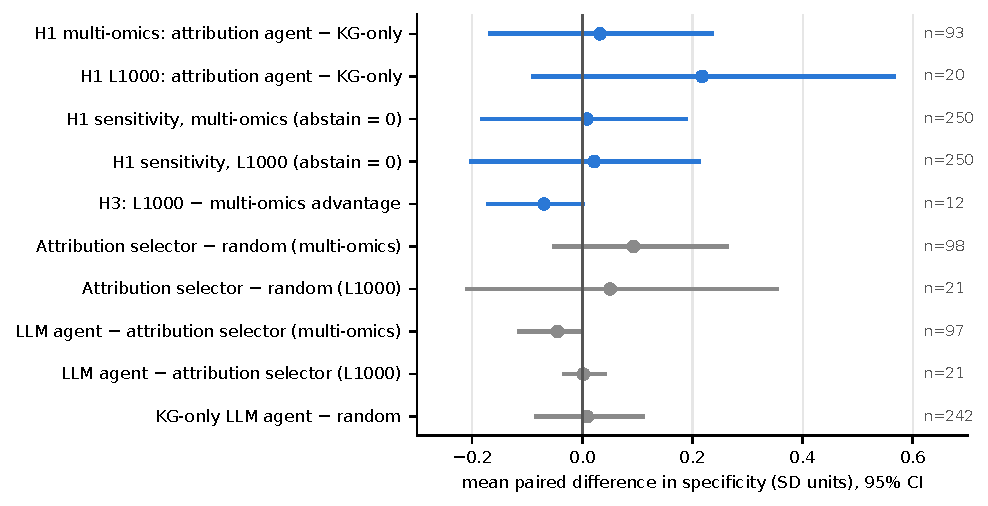
\includegraphics[width=0.92\linewidth]{fig_forest.pdf}
\caption{All paired comparisons on the synergy stratum. Blue: pre-registered (H1, H3); grey: exploratory. Points are
mean differences in dependency specificity (SD units) with 95\% cluster-bootstrap CIs. Every interval contains zero
except the LLM-agent-minus-selector comparison (multi-omics), which favours the selector.}
\label{fig:forest}
\end{figure}

H1 is not supported for either variant (Table~\ref{tab:h1}, Figure~\ref{fig:forest}). For multi-omics the effect is
essentially zero ($d_z = 0.04$), and its CI excludes effects larger than about $+0.23$ SD. For L1000 the point
estimate is larger ($+0.22$ SD), but it rests on 20 items from 17 cell lines and its CI includes zero. Scoring
abstentions as zero (all 250 items) or using the top-3 pathways does not change the verdict.

\subsection{Secondary hypotheses H2 and H3}

\begin{table}[h]
\centering
\small
\caption{H2 (does the attribution advantage differ between synergy and antagonism?) and H3 (is it larger for
L1000?).}
\label{tab:h2h3}
\begin{tabular}{@{}llrrrr@{}}
\toprule
Hypothesis & Variant & $n$ & Estimate & SE / 95\% CI & $p$ \\
\midrule
H2: attribution $\times$ synergy interaction & Multi-omics & 678 & $+0.058$ & 0.101 & 0.57 \\
H2: attribution $\times$ synergy interaction & L1000 & 520 & $+0.339$ & 0.270 & 0.21 \\
H3: $\Delta_{\text{L1000}} - \Delta_{\text{multi-omics}}$ & both & 12 & $-0.070$ & [$-0.17$, $+0.00$] & 0.12 \\
\bottomrule
\end{tabular}

\end{table}

Neither is supported (Table~\ref{tab:h2h3}). For H3 the point estimate even runs the other way (L1000 advantage
smaller than multi-omics by 0.07 SD), but it rests on only 12 shared items.

\subsection{Where the signal is lost: attributions vs the LLM (exploratory)}

\begin{table}[h]
\centering
\scriptsize
\caption{Decomposition with deterministic, no-LLM controls (synergy stratum). The selector picks the
highest-scoring admissible pathway; ``random'' is the expected score of a uniform choice among convergent pathways.}
\label{tab:decomp}
\resizebox{\linewidth}{!}{\begin{tabular}{@{}lrrrcrrr@{}}
\toprule
Comparison & $n$ items & Cell lines & Mean $\Delta$ & 95\% CI & $d_z$ & $p_{\text{mixed}}$ & $p_{\text{Wilcoxon}}$ \\
\midrule
\multicolumn{8}{@{}l}{\emph{What the attributions add (no LLM)}} \\
\quad Attribution selector $-$ random (multi-omics) & 98 & 33 & $+0.093$ & [$-0.05$, $+0.26$] & $+0.12$ & 0.29 & 0.62 \\
\quad Attribution selector $-$ random (L1000) & 21 & 18 & $+0.051$ & [$-0.21$, $+0.35$] & $+0.08$ & 0.53 & 1.00 \\
\multicolumn{8}{@{}l}{\emph{What the LLM adds on top of the same input}} \\
\quad LLM agent $-$ attribution selector (multi-omics) & 97 & 33 & $-0.045$ & [$-0.11$, $-0.00$] & $-0.16$ & 0.21 & 0.050 \\
\quad LLM agent $-$ attribution selector (L1000) & 21 & 18 & $+0.002$ & [$-0.03$, $+0.04$] & $+0.03$ & 0.90 & 0.65 \\
\quad KG-only LLM agent $-$ random & 242 & 41 & $+0.009$ & [$-0.08$, $+0.11$] & $+0.01$ & 0.78 & 0.62 \\
\bottomrule
\end{tabular}
}
\end{table}

Table~\ref{tab:decomp} separates the two places a signal could enter.
\begin{enumerate}
\item \textbf{The attributions.} Selecting the pathway by attribution score is not reliably better than a random
  convergent pathway ($+0.09$ SD, $p = 0.29$, multi-omics; $+0.05$ SD, $p = 0.53$, L1000).
\item \textbf{The LLM's choice.}
  \begin{itemize}
  \item With attributions, the agent does slightly \emph{worse} than the selector it is given (multi-omics
    $-0.045$ SD, CI $-0.11$ to $-0.003$, Wilcoxon $p = 0.05$; mixed model $p = 0.21$).
  \item Without attributions, the KG-only agent is indistinguishable from a random convergent pathway ($+0.01$ SD,
    $p = 0.78$).
  \end{itemize}
\end{enumerate}
So the null is upstream of the LLM: there is no dependency signal in the attribution-supported pathways for any
agent to find.

\subsection{What the agents claimed}

\begin{table}[h]
\centering
\scriptsize
\caption{Properties of the claimed top-1 pathways. Common-essential fraction: the share of the pathway's genes that
are DepMap common-essential. Diversity: distinct pathways named divided by items with a claim.}
\label{tab:pathways}
\resizebox{\linewidth}{!}{\begin{tabular}{@{}llrrrr@{}}
\toprule
Condition & Stratum & Mean spec (top-1) & Common-essential fraction & Pathway diversity & Median pathway size \\
\midrule
Attribution agent (multi-omics) & antagonism & $-0.003$ & 0.38 & 0.26 & 139 \\
Attribution agent (multi-omics) & synergy & $-0.024$ & 0.34 & 0.33 & 139 \\
\addlinespace
Attribution agent (L1000) & antagonism & $-0.046$ & 0.23 & 0.78 & 183 \\
Attribution agent (L1000) & synergy & $+0.046$ & 0.28 & 0.86 & 181 \\
\addlinespace
KG-only agent & antagonism & $+0.081$ & 0.33 & 0.17 & 139 \\
KG-only agent & synergy & $-0.018$ & 0.26 & 0.20 & 160 \\
\addlinespace
Attribution selector (multi-omics) & antagonism & $+0.031$ & 0.37 & 0.26 & 139 \\
Attribution selector (multi-omics) & synergy & $+0.011$ & 0.35 & 0.31 & 139 \\
\addlinespace
Attribution selector (L1000) & antagonism & $-0.046$ & 0.23 & 0.78 & 183 \\
Attribution selector (L1000) & synergy & $+0.044$ & 0.28 & 0.81 & 181 \\
\addlinespace
Random convergent pathway & antagonism & $+0.050$ & 0.32 & -- & 139 \\
Random convergent pathway & synergy & $-0.032$ & 0.27 & -- & 139 \\
\bottomrule
\end{tabular}
}
\end{table}

The KG-only agent concentrated on fewer pathways (diversity 0.17--0.20) than the attribution agents (0.26--0.86), so
it falls back on a few familiar convergent pathways when given no other signal. Mean specificity of the claimed
pathway is near zero in every condition. Their common-essential fractions are similar (0.23--0.38), so neither
condition simply picks pathways that are essential everywhere (Table~\ref{tab:pathways}).

\section{Interpretation}
\label{sec:interpretation}

\begin{itemize}
\item \textbf{The KG constraint works; the attributions do not inform.} The design goal of preventing hallucinated
  mechanisms was met: almost every claim is a verified KG path, and the agent abstains when nothing is admissible.
  But a constrained explanation is only as informative as its constraint. Attribution-supported pathways are no
  better at locating cell-line-specific dependencies than random convergent pathways.
\item \textbf{Why attributions carry no mechanism here.}
  \begin{itemize}
  \item SynergyLM sees 59 distinct cell profiles through 27,606 omics features. Dropping any one modality leaves
    test $r$ unchanged (0.764--0.765), and dropping all three costs 0.21.
  \item The follow-up study (SynergyLM-v2) tested this directly: replacing the omics encoder by a one-hot cell
    embedding makes no difference even for unseen drugs (median per-drug $\Delta r = -0.008$, $p = 0.48$).
  \item Reactome pathway features of drug targets perform no better than a structure-matched random-pathway control
    ($\Delta r = +0.002$, $p = 1$).
  \end{itemize}
  The omics act as a cell-line identifier, so gene-level attributions describe \emph{which} cell line it is rather
  than \emph{why} the pair synergizes.
\item \textbf{The expression confound (threat T1) was visible early.} In a pre-run smoke test on two items, the
  attribution-supported pathways overlapped substantially (Jaccard 0.27 and 0.48) with the pathways enriched when
  the ``attribution'' was just the cell line's expression deviation from the mean profile. Attribution support is
  therefore partly expression-driven.
\item \textbf{Implication for the extension.} A larger or paid LLM would not rescue H1, because the deterministic
  selector shows the signal is absent before any LLM sees it. Pathway-level explanations would need a model whose
  cell-side representation is not reducible to identity, or ground truth tied to the combination rather than to
  single-gene dependency (threat T4).
\end{itemize}

\section{Limitations and threats to validity}
\begin{itemize}
\item \textbf{Power.} Complete-case H1 has 93 (multi-omics) and 20 (L1000) items rather than the planned 240. The
  multi-omics null is informative (CI upper bound $+0.23$ SD); the L1000 null is not.
\item \textbf{Ground truth.} Single-gene CRISPR dependency of a pathway is a proxy: a pathway can be essential in a line
  without mediating the combination (T4).
\item \textbf{Coverage.} 41 of 59 cell lines have DepMap CRISPR data, and 29 of 129 drugs have no protein target
  (mostly cytotoxics), so the claim is restricted to targeted agents in covered lines.
\item \textbf{One LLM.} The study used one open-weight model. The decomposition argues that model choice is not the
  limiting factor, but other LLMs were not run.
\item \textbf{L1000 signatures} are consensus profiles from other cell lines, not the DrugComb line (T6).
\end{itemize}

\sloppy
\section*{Reproducibility}
\begin{itemize}
\item \textbf{Code:} branch \texttt{synergylm-v2}, commit \texttt{93de460} (``attribution-guided pathway explanation
  study''). Entry point \texttt{explain\_pathways.py} with stages \texttt{download, labels, map, kg, predict, sample,
  attribute, pathways, select, agent, score, analyze, gates}. Library: \texttt{src/explain/}. Tests:
  \texttt{tests/test\_explain.py}.
\item \textbf{Jobs:} \texttt{run\_xai\_train.sh} (models), \texttt{run\_xai\_pipeline.sh} (attributions, pathways,
  G0/G1), and \texttt{run\_xai\_agent.sh}. The last serves the LLM with vLLM, runs the 20-item pilot and gate G2,
  then the full agent run, scoring and analysis.
\item \textbf{Results:} \texttt{data/xai/results/analysis.json} and \texttt{scored.csv} (3,000 rows: 6 conditions
  $\times$ 500 items). Agent transcripts are in \texttt{data/xai/agent/}, and the failed pilot 1 is archived in
  \texttt{data/xai/agent\_archive/}.
\item \textbf{This report:} \texttt{reports/llm\_interpretation/}. \texttt{make\_tables.py} regenerates every table
  and the figure from \texttt{analysis.json}.
\end{itemize}

\end{document}
